\documentclass{beamer}% {{{
\usepackage{amssymb, latexsym, amsmath, graphics, fullpage, epsfig, amsthm, relsize, pgf, tikz, amsfonts, makeidx, latexsym, ifthen, hyperref, calc}
%\usepackage{eucal} this is a different font than \mathcal{•}
\usetikzlibrary{arrows}
%\newtheorem{theorem}{Theorem}[section]
\newtheorem{remark}{Remark}[section]
%\newtheorem{corollary}{Corollary}
%\newtheorem{lemma}{Lemma}
\newtheorem{assumptions}{Assumptions}[section]
\newtheorem{proposition}{Proposition}
%\newtheorem{definition}{Definition}
\newtheorem{notation}{Notation}
\usepackage{mathrsfs}
%\usepackage[shortlabels]{enumitem}
\usepackage{tikz}
\usepackage{amsmath}
\usetikzlibrary{arrows}
\usetikzlibrary{shadows.blur}
\usepackage{pgfplots}
\usepackage{mwe} % For dummy images
\usepackage{subcaption}
\usepackage{multirow}
\usepackage{dcolumn}
\newcolumntype{2}{D{.}{}{2.0}}
\usepackage{multicol}
\numberwithin{equation}{section}

\newcommand{\lip}{\textup{Lip}_b}
\newcommand{\liph}{\text{Lip}_{\hat\rho}}
\newcommand{\R}{\mathbb{R}}
\newcommand{\E}{\mathbb{E}}
\newcommand{\Norm}[1]{\left\|  #1   \right\|}
\newcommand{\ud}{\ensuremath{\mathrm{d} }}

\newcommand{\mySeparateLine}{
	\begin{center}
		\makebox[\linewidth]{\rule{0.6\paperwidth}{0.4pt}}
\end{center}}
%\usepackage{lipsum}%% a garbage package you don't need except to create examples.
%\usepackage{fancyhdr}
%\pagestyle{fancy}
%\lhead{\Huge Version A}
%\rhead{\thepage}
%\cfoot{}
%\renewcommand{\headrulewidth}{0pt}



\setbeamersize{text margin left=2mm,text margin right=2mm}

\usepackage{animate}

\usepackage{tikz}
\usepackage{pgfplots}
\pgfplotsset{compat=newest}
\usetikzlibrary{decorations.markings}

\allowdisplaybreaks


\defbeamertemplate{footline}{higher page number}
{%
	\hfill%
	\usebeamercolor[fg]{page number in head/foot}%
	\usebeamerfont{page number in head/foot}%
	\insertframenumber\,/\,\inserttotalframenumber\kern1em\vskip20pt%
}
\setbeamertemplate{footline}[higher page number]

% }}}
% {{{ Title page
\title[About Beamer] %optional
{Graduate Seminar \\
An introduction to stochastic calculus with applications to finance and SPDEs}

\author[Arthur, Doe] % (optional, for multiple authors)
{Nicholas Eisenberg}


\date[VLC 2021] % (optional)
{ \small March 29, 2022 
}

\logo{\includegraphics[height=1cm]{overleaf-logo}}
\thispagestyle{empty}

\begin{document}
	\frame{\titlepage}	
	\setcounter{page}{1}
	\begin{frame}{Stochastic Calculus}
In Real Analysis we study measurable functions:
	\[
		f : D \to R,
	\]
where both $D$ and $R$ are measurable spaces:
	\[
		(D, \sigma(D), \mu_1) \quad \text{and} \quad (R, \sigma(R), \mu_2).
	\]
In undergraduate Calculus, we focus only on real valued measurable on $\R^d$:
	\[
		f : D \subseteq \R^d \to \R^d,
	\]
and the measure space that is implies is the following:
	\[
		(\R^d, \mathscr{B}(\R^d), \lambda),
	\]
where $\lambda$ is Lebesgue measure.
	\end{frame}

	\begin{frame}{Stochastic Calculus}
When studying Stochastic Calculus, and in general  Probability Theory, we consider measurable functions,
	\[
		X : \Omega \to \R^d,
	\]
and we consider the measure spaces 
	\[
		(\Omega, \mathcal{F}, \mathbb{P}) \quad \text{and} \quad (\R^d, \mathscr{B}(\R^d), \lambda),
	\]
where $\Omega$ and $\mathcal{F}$ are referred to as the sample space and set of possible events and
	\[
		\mathbb{P}(\Omega) = 1.
	\]
\begin{definition}[Random Variable]
	A measurable function $X: \Omega \to \R^d$ is called a {\it $\R^d$-valued Random Variable}.
\end{definition}

So essentially, Stochastic Calculus and Probability is just Real Analysis on Random Variables. 
	\end{frame}

\begin{frame}{Stochastic Processes}
	\begin{definition}[Stochastic Process]
A stochastic process is a random variable that is indexed by set, $T$, which usually represents time:
	\[
		X_t(\omega), \quad t \in T, \; \omega \in \Omega.
	\]
One can think a stochastic processes as a two parameter function
	\[
		X_t(\omega) = X(t,\omega): T \times \Omega \to \R^d.
	\]
	\end{definition}
	\begin{definition}[Sample Path]
The variable $\omega$ represents the idea of a single possible outcome. The following function is then referred to as a {\it sample path}:
	\[
		t \mapsto X_t(\omega).
	\]
	\end{definition}

\end{frame}

\begin{frame}{Examples}
	\begin{example}
Suppose we leave a cup out in the rain. We may model this with a stochastic processes as 
	\[
		X_t(\omega) = \text{Amount of rain in the cup at time $t$}.
	\]
Since $X_t \ge 0$, maybe we could say that 
	\[
		X_t \sim \text{Gamma Distribution with } \mu := \mu(t) \text{ and constant variance } \sigma^2
	\]
	\end{example}
If the rain is constant then it makes sense for the variance to be constant. Moreover, as time continuous, there will be more water in the cup on average, so the mean should be a function in time.
\end{frame}

\begin{frame}{Brownian Motion.}
Brownian motion is a very widely used stochastic processes. We will construct Brownian motion through a random walk.

\begin{Theorem}
	Consider a random walk $X = \{X_{0}=0, X_{t_1}, \cdots, X_{t_n}\}$. Suppose that for $k \in \{1, \cdots ,n\}$ that
		\[
			\mathbb{P}\left[ X_{t_k} = -h \right] = \mathbb{P}\left[ X_{t_k} = h \right] = 1/2.
		\]
	and suppose that the time increments are all constant:
		\[
			t_k-t_{k-1} = d \quad \forall k \in \{ 1, \cdots, n \}.
		\]
	Suppose that $h^2 = d$. Now define 
		\[
			B_n(t_{k}) = \sum_{i=0}^k X_{t_i}.
		\]
	Then $B_n$ converges to a Brownian motion. 
\end{Theorem}
\end{frame}

\begin{frame}{Random Walk Example}
\begin{center}
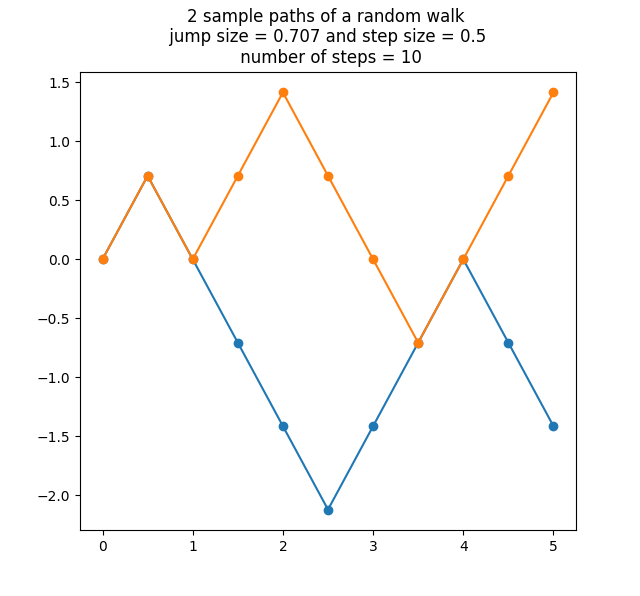
\includegraphics[scale=.6]{randomwalk1.png}
\end{center}
\end{frame}

\begin{frame}{Random Walk Example}
	\begin{center}
		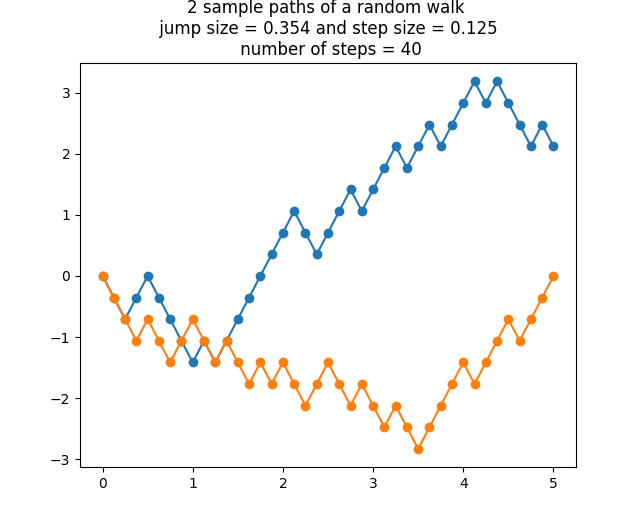
\includegraphics[scale=.6]{randomwalk2.png}
	\end{center}
\end{frame}

\begin{frame}{Random Walk Example}
	\begin{center}
		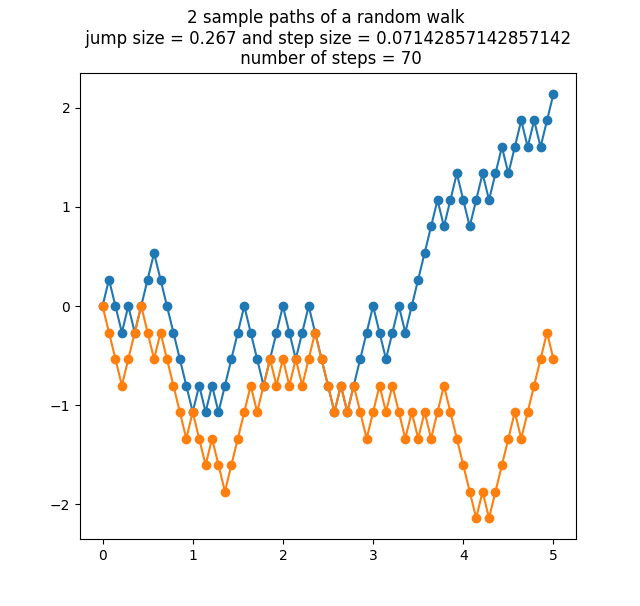
\includegraphics[scale=.55]{randomwalk3.png}
	\end{center}
\end{frame}

\begin{frame}{Random Walk Example}
	\begin{center}
		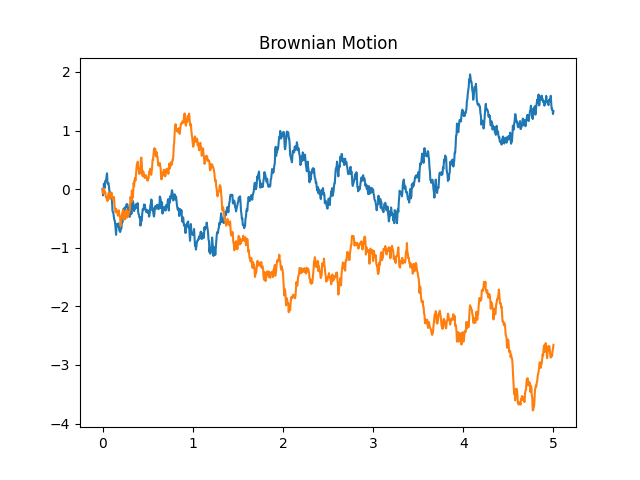
\includegraphics[scale=.7]{BrownianMotion.png}
	\end{center}
\end{frame}

\begin{frame}{Why do we care about Brownian Motion? An application to finance.}
	Consider a stock that has value $S_t$ at time $t$. Consider $t=0$ to be the point of entry into the investment. We can define a return rate as follows:
		\[
			S_t = S_0(1 + R_t ), \quad R_t = \text{ the return rate over the period $[0,t]$} .
		\]
	We want to make predictions of our return. In a very simple model, we can assume that 
		\[
			R_t \sim \text{Normal}(\mu t, \sigma^2), \quad \mu \in \R,\; \sigma \in (0,\infty).
		\]
	In terms of Stochastic Calculus, we express this as the following stochastic differential equation:
		\[
			dS_t = \mu S_t \ud t + \sigma S_t \ud B_t, \quad \text{where } B_t \text{ is a Brownian motion.}
		\]
	
\end{frame}

\begin{frame}{Modeling a stock price with geometric brownian motion}
The notation 
	\[
		dS_t = \mu S_t \ud t + \sigma S_t \ud B_t, \quad \text{where } B_t \text{ is a Brownian motion}
	\]
is only symbolic as $dB_t$ does not exist. The above can be legitimately viewed as the following integral equation:
	\[
		S_t - S_0 = \int_0^t \mu S_k \; \ud k + \int_0^t \sigma S_k \; \ud B_k.
	\] 		
The stochastic processes $S_t$ that solves the above equation is called a Geometric Brownian Motion. 
\end{frame}
	
	\begin{frame}
		\frametitle{References}
		\small
		
		\begin{thebibliography}{999}
	
		\end{thebibliography}
	\end{frame}

\end{document}
